\chapter{Software Design, Implementation and Testing}

\section{Requirements}
There are two main components to the software being developed for this project. The first is the manipulation of the data into a database, and the second is a web front end for the data to be accessed via. 

\subsection{Database}
The database has to store the following information for each hit from the alignment with \textit{C. albicans}:

\begin{itemize}
  \item ID of the hit that was found when the species coding sequences have been aligned with \textit{C. albicans}.
  \item Species it came from.
  \item The gene name and ID from Candida Genome Database.
  \item UniProt ID.
  \item Contig of raw DNA.
  \item Coding sequence of nucleotides.
  \item Amino Acid (protein) sequence that the coding sequence codes for.
  \item Annotations from NCBI nr database to provide a description of the proteins.
  \item A list of Gene Ontology\cite{geneontology} ID's for the protein.
  \item If it can be found, the positions of the start and end of the coding sequence in the raw contig. 
\end{itemize}

From these requirements it is clear there are a few pieces of data that need to be extracted from the data that has been collated. For each alignment with \textit{C. albicans} the protein sequence and GO annotations need to found, the coding sequence that was used in the alignment and the contig that it came from. In addition to this, the metadata about the genes such as the name and ID's need to be read from the mapping file that was created earlier. 

The final bit of data that needs to be added is the position of the coding sequence in the contig. An algorithm will have to be developed to detect this.

\subsection{Website}
The website will only have a few funcitonal requirements: 

\begin{enumerate}[label=FR\arabic*]
  \item Display each record in the database in an easy to read manner. 

    The first requirement, is that each document in the database can be accessed, and presented to the user. It will have to display all of the fields of the document without overwhelming the user, this is a risk as some of the sequences are very large. Links to other databases such as the Gene Ontology database, and UniProt database will have to be made into hyperlinks for the user to easily navigate to the relevant information for the found gene. 

  \item Highlight coding sequence in contig if possible.

    Visually representing the coding sequence inside of the raw assembled contig, is helpful for researchers to see the surrounding bases up and down stream of the coding sequence. It also allows them to see the full coding sequence with any introns (non-coding regions of bases) included. 

  \item Copy coding sequence and +/- a user defined number of bases to the clipboard.

    The user should also be able to copy the coding sequence to their clipboard, for use in other applications. They should also be able to select a number of bases to be copied that surround the coding sequence. 

  \item Search the database for a gene, by name, description, ID, or even by nucleotide sequence. 

    The search functionality is the main feature of the site as it is what takes the previously difficult to use data, and makes it truly accessible. 
\end{enumerate}

\section{Design}

\subsection{Choice of Database Technology}
The first stage in designing this system was to decide upon what database technology would be used for the data store. In the Analysis section the merits and disadvantages of NoSQL and SQL solutions were highlighted in generic terms. For this project there is a focus on using modern web development technologies, and MongoDB (A NoSQL database solution) fits this well, as it stores data based on use case, which fits well with the MVC design pattern, as typically each Model in the design refers to a use case. 

In this project there will only be one set of data to be stored, the list of genes and their various related data. From the users perspective they will only be interacting with this set of data, they will never be trying to combine a gene with another dataset for example. The only use case for this data then is for it to be displayed. 

If this data was stored in a relational system like PostgreSQL, then there would need to be several tables for shared data, to store it in a normalised form. For example, there would be a contig table and each gene would store a link to the contig that it was from. This means that when a user requests to view a gene, the database will have to perform a join between the gene table and the table storing the contig to retrieve all of the relevant information. This makes it harder to develop and maintain the database, as the relations between the datasets have to be considered throughout the project. 

This would be advantageous if the data was going to be updated frequently, as a piece of data only needs to be updated once, as it is only stored once. However as this project is effectively read only, the data is never going to change, this isn't an issue with a NoSQL solution.

This choice was also influenced by the choice of server side language, which for this project will be Node.js. 

\subsection{Choice of Server Side Technology}
`Node.js is a JavaScript runtime built on Chrome's V8 JavaScript engine. Node.js uses an event-driven, non-blocking I/O model that makes it lightweight and efficient. Node.js' package ecosystem, npm, is the largest ecosystem open source libraries in the world.'\cite{node-org}

Node.js was chosen for several reasons, firstly as both server side and client side portions of the code are written in JavaScript, it is easier to develop, since you are working with one unified language. Rather than having to learn to use and build a server side language as well as JavaScript.

It also works very well with MongoDB, as MongoDB represents it's data as JSON objects, which are native to JavaScript. This makes querying and operating on data returned via MongoDB much easier, as it is already in a format native to the language. 

Node.js has a very good packaging system, called Node Package Manager (npm), the npm repository has access to the largest collection\cite{modulecounts} of software packages, as well as being very easy to use and maintain thanks to the package.json file, which is automatically updated when new modules are used. 

JavaScript has historically been looked down on due in part to it's syntax and type system, however with the latest stable specification\cite{es6} (ES6) of the language, a lot of these issues have been addressed. 

As outlined in Ioannis K. Chaniotis et al's paper, `A study on the viability of Node.js for web development from the perspective of performance.', they conclude that `... Node.js offers client-server development integration, aiding code reusability in web applications, and is the perfect tool for developing fast, scalable network applications.'\cite{node-perf}

In addition to this, prior work has been done with the language on several projects, which reduces the barriers to development that learning a new language would create. 

\subsection{Nodestack}
The project will be utilising a set of boilerplate code called Nodestack\cite{nodestack}. This code helps to setup a basic web service and provides many extra features to compliment the basic Node.js stack. 

\subsubsection*{ES6}

    Since Node.js version 4.0, it has supported the ES6 standard, which provides a lot of syntactic sugar, and makes the formatting of the code a lot easier to read and write. This is also supported for the client side code via the babel transpiler, which compiles ES6 code into the more widely supported ES2015 standard.

    \subsubsection*{Webpack}
    
    Webpack is a module bundler that allows for easy packaging of client side JavaScript. It allows the client side JavaScript to be written in ES6, then when built it will transpile the ES6 code into more widely supported ES2015 code, minify it for efficiency, and package it into one single file. This means that the code can be written in a nicely organised manner across multiple files in ES6, and then reduced to one small and widely supported file, for actual usage in production.

    \subsubsection*{Mongoose}

    Mongoose is an Object Data Manager, it allows developers to define schemas and validation for their data objects as well as extensible models for those objects. This makes interactions with MongoDB a lot simpler, as well as easy enforcement of validation rules.

    \subsubsection*{Pug}

    Pug is an HTML templating language that allows developers to write HTML with dynamic variables from the server side, and include some logic elements. The main benefit is that it has a much cleaner syntax than HTML so it is a lot easier to read and write. 

    \subsubsection*{Stylus}

    Stylus is an expressive CSS language that, like Pug and ES6, improves the syntax of CSS by minimising unnecessary elements. It has many other advantages over CSS, although for this project they aren't likely to be utilised as the front end design work of this project will be minimal. 

    \subsubsection*{Bootstrap}

    Bootstrap is a CSS and JavaScript framework that is aimed at making responsive websites easier to write. With the addition of bootstrap to the project, adapting the front end to work on mobile will be a minimal amount of work. It also adds useful features for laying out the page and some attractive default CSS. 

Using this boilerplate will save a huge amount of time in development as the basic framework of the web application is already laid out, so the development time can be focussed on developing software to meet the functional requirements rather than investing time in setting up a good web framework. 

For more detail on how the boiler plate works, you can read the guide here: \url{http://blog.owen.cymru/nodejs-es6-boiler-plate/}

\section{Build Process}
  One of the first things that was setup for this project was the build process. This doesn't take long to setup but provides a huge benefit for the rest of the project. It helps to reduce errors and speed up the process of deployment and testing.

  \subsection{Development Environment}
    This project will be developed on an Arch Linux system, as it will only ever be ran on a Linux host this isn't an issue, as the production hosts' architecture will match the development one. 

    All of the code and LaTeX for the report will be written with the Vim text editor, which has been configured to have many optimisations to this workflow. The full Vim configuration that was used can be found here\cite{vimrc}.

  \subsection{Code Style}
  For this project the Clock Limited code standard\cite{clockstandard} will be followed. This has a few key variations to typical Javascript. 

  \begin{itemize}
    \item Semicolons are not required in JS, so they are not used to denote end of line.
    \item Strings are encapsulated with single quotes, not double. 
    \item Comma first\cite{commafirst} listing of variables, objects and arrays.
    \item No commenting, to avoid confusion, encourage descriptive naming and reduce file length.
  \end{itemize}

  These rules ensure that the code written is clean and easy to read, something that is crucial for producing high quality and easily maintainable code. 

  \subsection{Version Control}
    This project is being entirely tracked with Git version control. This is to ensure that all of the work is backed up to a remote repository, with an easily accessible history. It also allows for branching of the project to test out experimental features or bug fixes. The project is remotely hosted on Github\cite{github} for remote backup and access via multiple hosts. Github is also widely supported by third party integrations, something that will be utilised quite extensively, in this build and deployment process tool chain.


  \subsection{Test Suite}
  When pushing code to Github, a module called Husky\cite{husky} will run the test suite on the developers local machine.

    The test suite is set up to first clean the project of old builds and coverage reports, then run ESlint\cite{eslint}. This will scan the entire codebase for files that do not adhere to the code style. This means that any badly formatted code will cause an error and prevent the code from being pushed until the issues are fixed.

    After the linting check, the test suite will use Mocha\cite{mocha} to run all of the JavaScript test files that are in the project. If any of the assertions made in the test files fail, the project will not be pushed. 

    Once the test's have been ran Istanbul\cite{istanbul} will provide a coverage report, that will show to the user the percentage of tested code that has been covered by the assertions. After this the code can finally be pushed to Github. 
    
  \subsection{Continuous Integration}
    Once the code has been pushed to Github, a hook on Github will trigger Travis CI\cite{travis} to clone down the latest version of the code to it's servers and run the test suite again on it's own server. This is very useful as occasionally developers can bypass Husky to push code, or have something setup in their system that isn't defined in the application, that causes tests to pass on their system but not when the application is built from scratch. The CI test will expose any bugs that arise from these situations and prevent the code being deployed to the staging server. 

    Once those tests are successful, it will send the coverage report generated by Istanbul to another third party service called Codecov\cite{codecov}. This tracks the test coverage over time and provides interactive charts highlighting areas that need more test coverage. 

\begin{figure}[H]
\begin{center}
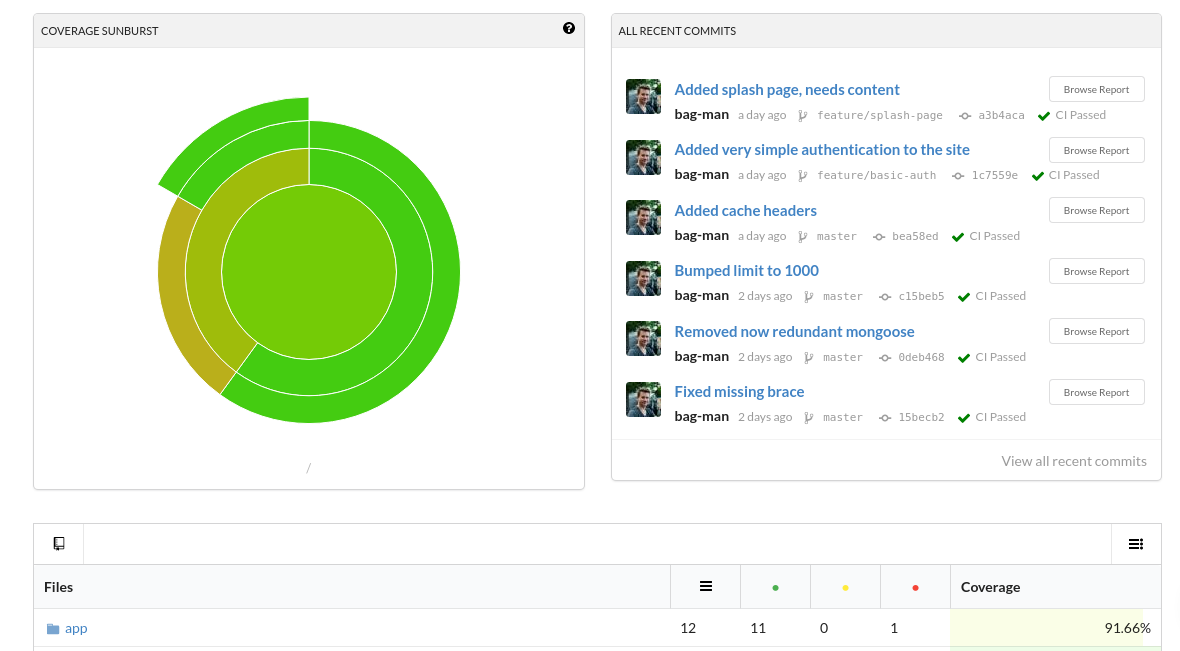
\includegraphics[scale=0.3]{codecov}
\caption{Codecov interactive coverage report}
\end{center}
\end{figure}


  \subsection{Deployment to Staging}
  If the tests pass on Travis CI, a Github hook will then activate the staging deployment. The project is setup to use Heroku\cite{heroku}, and to build on successful CI results. This means that when code is pushed to the master branch, it will automatically be deployed to their service. This is excellent for development as it allows changes made to the system to be almost immediately reflected on the staging website. The only drawback of Heroku is that this project is using their free offerings which only allow 500MB's of database storage, which means that anything larger than that will be truncated. 

  The benefits of this build process are clear, firstly code is automatically deployed, which saves time as deployments don't have to be done manually, as well as encouraging regular client feedback. However the main advantage is that before the deployment the code will have had the test suite ran on it twice, once on the developers local machine and then again on a brand new build on the CI service. This means that any mistakes are caught before they are put into production and the developer is notified of these issues so they can't be avoided. 



\subsection{Database Import}
To import the data into the database from the FASTA file format, a script will be written that will use a module called fasta2json\cite{fasta2json} to read the fasta files into JSON format. 

From there it will use the alignment results generated by the Diamond script to look up the contig, coding sequence, and amino acid sequence (protein) for each of the alignment results. 

It will also compare the hit ID with the mappings file that was produced to get the ID's for the equivalent UniProt and Candida Genome Database hits, if they are available. 

A function to find the position of the coding sequence in the raw contig will then be ran, which will return the start and end positions of the coding sequence in the contig.

That data will then be inserted into MongoDB, and an index built on the searchable fields. This index will allow for a very fast and efficient search for the key fields that will be searched for in the database; description, gene name and ID's.

\begin{lstlisting}[caption=The database schema that will represent a gene in the database.]
  { id: Schema.ObjectId
  , hitid: String
  , species: String
  , name: String
  , cgdid: String
  , uniprot: String
  , contig: 
    { head: String
    , seq: String 
    }
  , codingseq: 
    { head: String
    , seq: String 
    }
  , protein: 
    { head: String
    , seq: String
    , goids: [String]
    , desc: String 
    }
  , codingRange: 
    { start: Number
    , end: Number
    , fail: Boolean 
    }
  }
\end{lstlisting}

    
\subsection{Website Architecture}
As the application only has one data object to model, the architecture isn't that complex. However it is still beneficial to follow good design principles which is why a traditional Model View Controller (MVC) design pattern\cite{mvc} was followed. 

The MVC design pattern allows for each data object that is being modelled to have three components, a model which defines the data's structure and it's functionality, a controller that is how the application interacts with that model, and finally a view, which is what is displayed to the user and how they interact with the model. For example a user may click on a gene, which sends a request to the controller, the controller then requests that gene from the model, which in turn updates the view, the user can then see the gene that they had selected. 

Abstracting the functionality of the project out into these three components allows for the development to be a lot easier to manage and work with, than having one monolithic class to handle the entire functionality of a gene object.

There will only be two routes in the application, one to the home page, which will simply display a splash page with some information about the website and project, and another route that handles searching and viewing genes.

When viewing a gene, the coding sequence will have to be highlighted inside of the contig. To do this the coding range that was determined when the data was imported will be used to select the substring, and then some client side JavaScript will modify the HTML to wrap the coding sequence inside of a span tag. 

As the coding sequences are stored in the database in only one compliment, there will be a reverse compliment button to reverse the compliment of the coding sequence. This is useful if the coding sequence is highlighted in the contig as the reverse compliment, it will allow the users to visually check that the data is correct. 

\subsection{User Interface}
Before building the user interface for this project, several other similar sites were examined to see what information they were displaying and how it was laid out. The first was the Candida Genome Database\cite{cgd} and it's locus page. It lists column headings on the left, and the information on the right. This design is easy to read and doesn't clutter up the page too much.

\begin{figure}[H]
\begin{center}
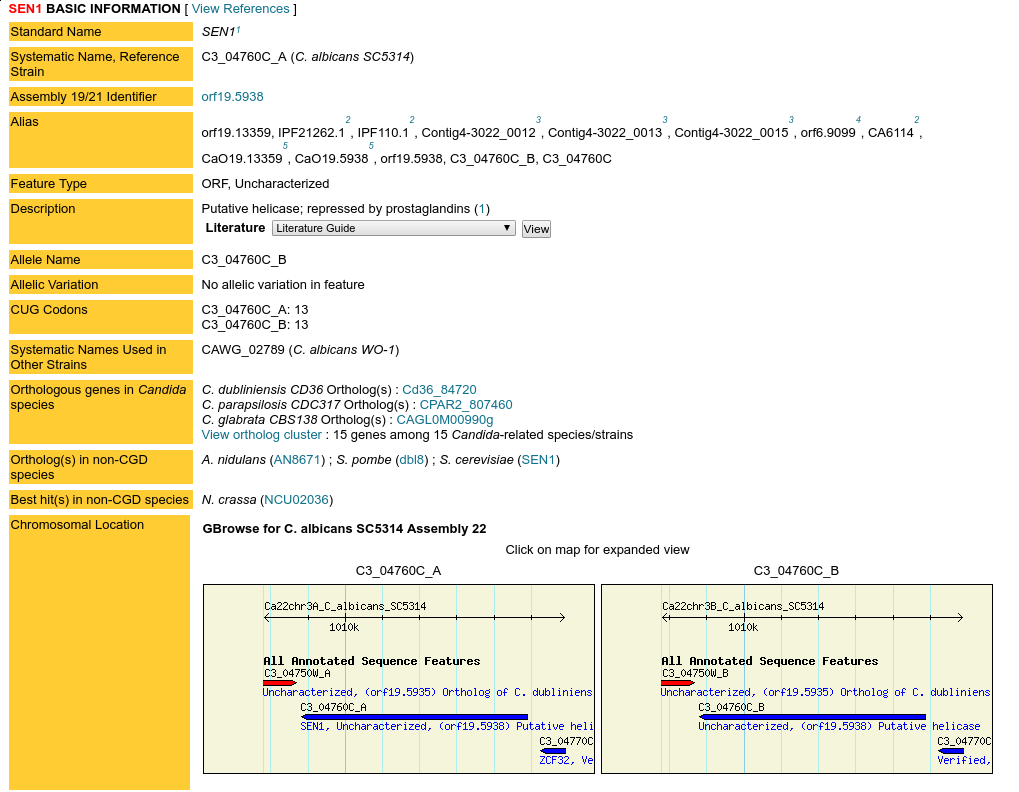
\includegraphics[scale=0.40]{cgd-locus}
\caption{Candida Genome Databases's locus page}
\end{center}
\end{figure}


\begin{figure}[H]
\begin{center}
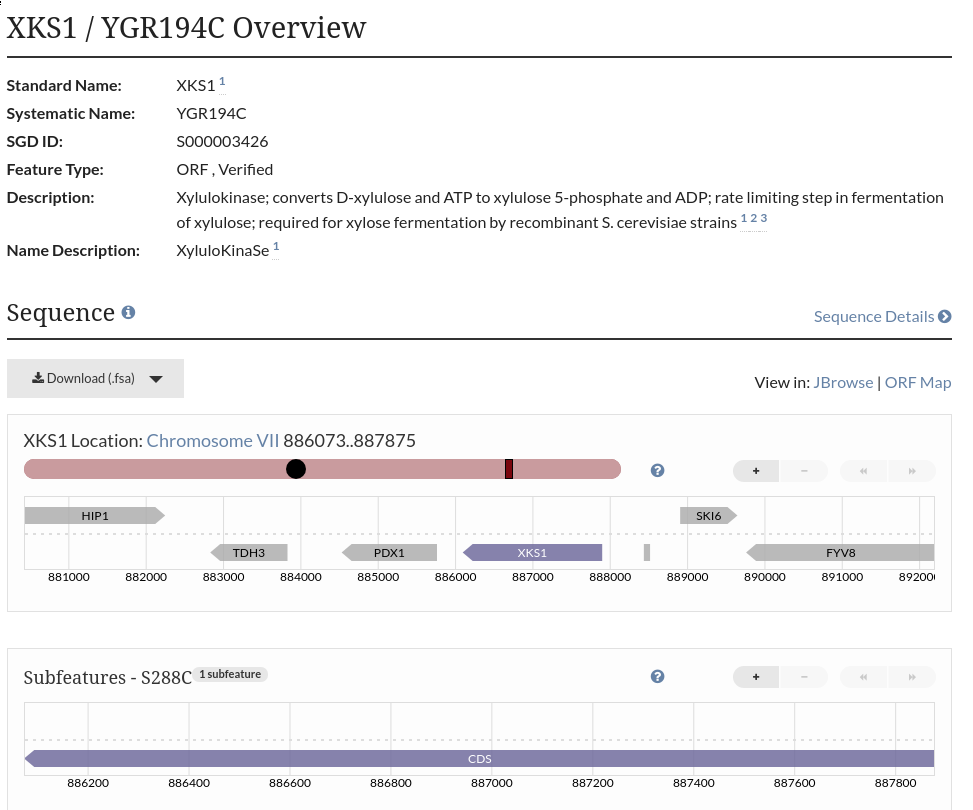
\includegraphics[scale=0.40]{sgd-locus}
\caption{Yeast Genome Project's locus page}
\end{center}
\end{figure}

Also examined was the Yeast Genome\cite{sgd} project's locus page. This page was very nicely formatted and laid out, it clearly had a lot of development, as it had integrations with two genome browsers as well as a large amount of extra information and graphical representations of the genes locations. Replicating this would be ideal, however it is too far out of the scope of this project, as many extra systems would have to be setup to get this data and make it as interactive.

Much like the rest of this project the UI was prototyped along with the understanding of the data at the time. This means that the UI was evolving with the data, and wasn't truly decided upon and polished until the data that was being displayed was known to be correct, and wouldn't change. Unfortunately this didn't happen until quite late in the project. 

\subsubsection{Final design}
The focus for this design was to make it as simple to implement and use as possible, as this isn't a public facing service it doesn't need to be a cutting edge design aimed at grabbing users attention. Instead it just needs to be functional and represent the data clearly. 

There are only two main pages on the website, a search view, and a locus page for specific genes. These share the same template, and adapt based on the data provided to them. The tasks for these pages are simply to display the data in the database, and provide a form to query it.

Tooltips were used to display information about each row. As the site is only going to be used by a couple of researchers there wasn't much benefit to creating a help section or a how to guide on how to use the site, as firstly it has been changing a lot during development and secondly it is quicker to just have a direct conversation with them about areas that they might not understand. However if in the future this were to become a public service, the home splash page would be updated to provide more information to external users.

The page was constructed with bootstraps\cite{bootstrap} grid system, which allows the content to be dynamically repositioned to fit different size displays.

\begin{figure}[H]
\begin{center}
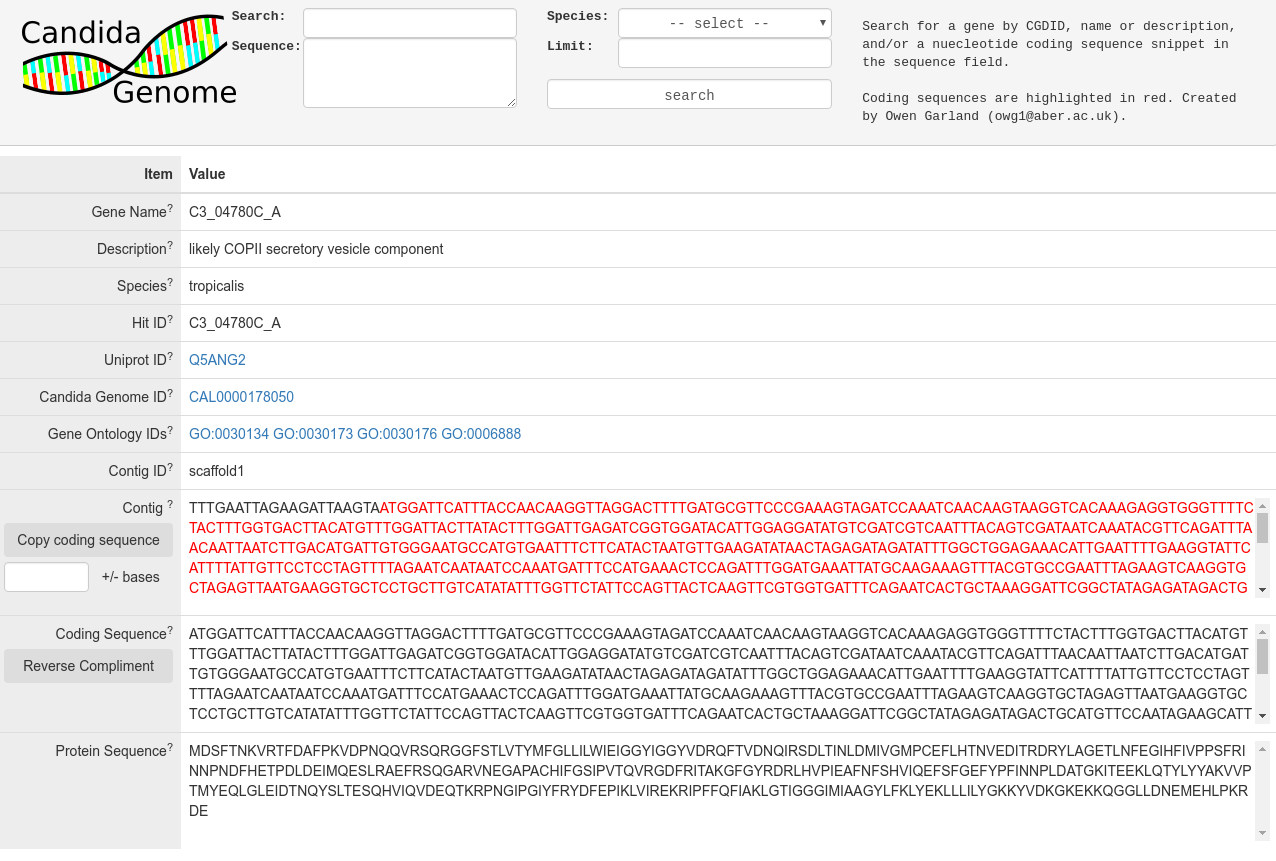
\includegraphics[scale=0.30]{candida-locus}
\caption{The final locus page for the project}
\end{center}
\end{figure}

\begin{figure}[H]
\begin{center}
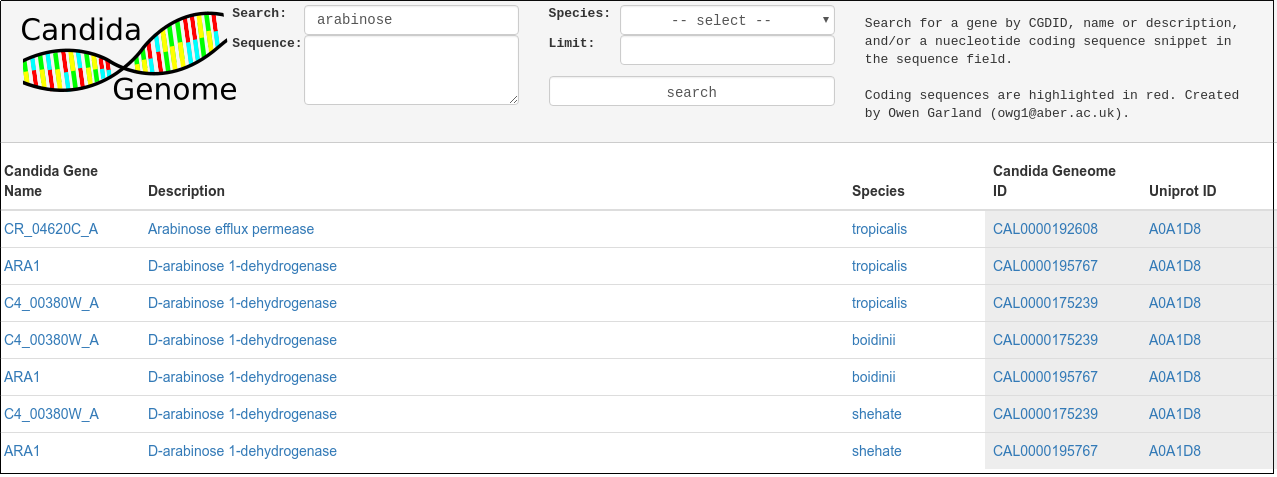
\includegraphics[scale=0.35]{candida-search}
\caption{The final search page for the project}
\end{center}
\end{figure}

\begin{figure}[H]
\begin{center}
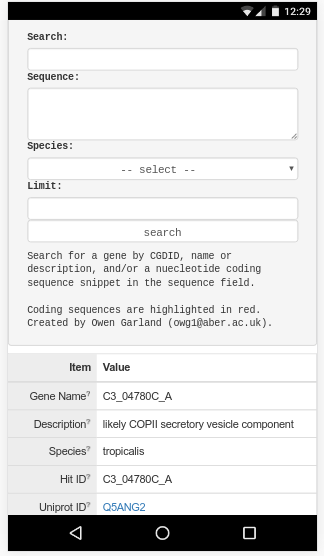
\includegraphics[scale=0.6]{candida-mobile}
\caption{A locus page viewed on a mobile device}
\end{center}
\end{figure}

\begin{figure}[H]
\begin{center}
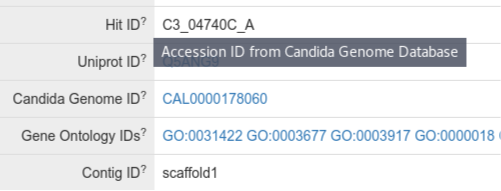
\includegraphics[scale=0.6]{candida-tooltip}
\caption{Tooltip on mouse hover describing what row means}
\end{center}
\end{figure}

\section{Implementation}
During the investigation into the data, many issues were encountered. Mainly due to a lack of understanding of what the data meant, and how it was produced. Initially the plan was to take the raw contigs for each species and use diamond to align them against the NCBI nr database. Then from those results link the data back to the Candida Genome Database via the RefSeq ID's that the NCBI nr database uses. However it was later discovered that there was an annotated set of aligned data in the provided data, meaning that this step was no longer necessary.

A prototype was built around this alignment data, however it was then realised that the data for \textit{C. boidinii} was not aligned against the NCBI nr database, but rather another unknown data set. This meant that to pursue this line of prototyping a replacement dataset for \textit{C. boidinii} would have to be made, or alternatively reproduce all three datasets with another pipeline, as the results from the alignments weren't consistent. 

The core problem was that it was unknown what tools had been used to produce this data as there was no accompanying documentation. It appeared that a proprietary tool blast2go\cite{blast2go} had been used to align and annotate the data. However after using a trial copy to try and replicate the results it was evident that this tool had not actually been used to create the alignments with the NCBI nr database. 

Eventually it became clear that the alignment had been performed with the BLAST tool, on the universities high performance cluster, with an XML format that wasn't known to have been an option at the time. This meant that the data could actually be reproduced quite easily with Diamond, using the newly discovered XML output that BLAST alignments offer.

After these revelations, and another meeting with the researchers, we discovered in the original datasets that there were in fact already annotated protein sequence files and coding sequence files.

\subsection{Collating the data, and linking it to Candida Genome Database}
This meant that the data was already processed and largely annotated already. There was however one missing piece which was the link back to the Candida Genome Database (CGD), something that would be invaluable to the researchers who were already familiar with the CGD. 

Because of this, thankfully the weeks of effort spent learning about alignments and annotations weren't wasted, as a new alignment was needed to be produced, using the coding sequences in the data set against the proteins found in \textit{C. albicans}, the latter being provided by CGD\cite{albicans}. 

This data generated was then able to be used to link the coding sequences found in the data sets to the well documented genes in \textit{C. albicans}. In addition to this the other annotations provided by the original dataset, such as Gene Ontology ID's, are able to be enhanced by using a mapping from the Candida Genome Database to get UniProt ID's which offer even more information on the known genes. 

Now each species had, the raw assembled contigs, the coding sequences, the amino acid sequences, the annotated protein information, a link to the Candida Genome Database, and in some cases a link to the UniProt database.


\subsection{Finding the coding sequence in the contig}
The next key piece of information to recover that would be of great use to the researchers was the position of the gene (coding sequence) inside the raw assembled contig. With this information they would be able to easily find the sequence of bases that surround the gene.

To do this mock data was produced manually, that contained the correct results, and unit tests made to check if a dummy function was returning the correct results as defined in the mock data. Then an algorithm was developed to find the position of a coding sequence inside a contig, using these tests to check the accuracy of the functions results.

The initial algorithm was only finding around fifty percent of the genes in the dataset. After some discussions with the project supervisor, it became apparent that the reason for this is that the coding sequences were stored in one compliment, but the alignment results were finding genes that were the reverse compliment. This explains why around fifty percent of the genes weren't found. 

Modifying the algorithm to search for the reverse compliment of the coding sequence if it wasn't found at first, resulted in every gene being detected. The algorithm, simply found the index of the first twelve bases of the coding sequence in the contig, and the last twelve bases of the coding sequence in the contig. If the start or end couldn't be found it was assumed that the gene was spread across two contigs and the start or end respectively were marked to indicate that the gene was split across two contigs. 

\begin{figure}[H]
\begin{center}
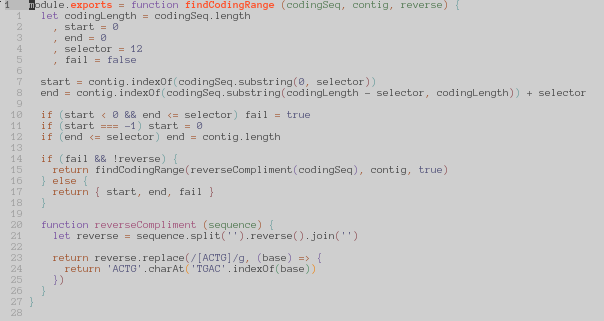
\includegraphics[scale=0.70]{code4}
\caption{Algorithm to find coding sequence inside a contig. \label{overflow}}
\end{center}
\end{figure}

\subsection{Search functionality}
Implementation of the search feature underwent several iterations, initially a search based on a regex match was implemented. This meant that each field was searched individually for any subset of the query string. This was very powerful as it would allow substrings to be found for each property of the searched for term. 

An example of this would be if `glucose-6' was searched in the description field, all documents in the database with that string in the description would be returned. This could then be combined with other fields to narrow down the query. 

This implementation was done during the prototyping phase to get a very basic search working for testing purposes, the reason it wasn't going to remain in the application, is that a project wide regex search is very inefficient as the search has to be matched against every value in the entire database for every single query made. This would have resulted in search operations on the website being too slow to be functional.

A better solution was to create a generic search field using MongoDB's textSearch\cite{textsearch} feature, that utilises pre-compiled indexes to lookup data in a far more efficient manner. The downside of this approach is that indexing is quite an intensive task, however for this application there is no new data being added to the system, nor is any data being modified once the system is running. This means that the intensive indexing stage only occurs once, at build time when the data is imported to the system.

The fields indexed for the text search are the gene name, protein description, UniProt ID and Candida Genome Database ID. Weights are then applied to each field to determine their value when sorting the results of a search. For example a match with a UniProt ID is weighted higher than a protein description, allowing for results that have a match to a UniProt ID to be displayed higher in the search results, than those without.

With this system in place the search was functioning very well, however there was an issue, if a search returned a large amount of documents back, the sort was unable to be ran due to the default MongoDB sort buffer limit being too small to handle the number of results returned. To get around this issue the search function was re-written as an aggregate function. Aggregate\cite{aggregate} in MongoDB allows for a pipeline of steps to be applied to a query, as well as the option to use disk if memory limits are reached. 

\begin{figure}[H]
\begin{center}
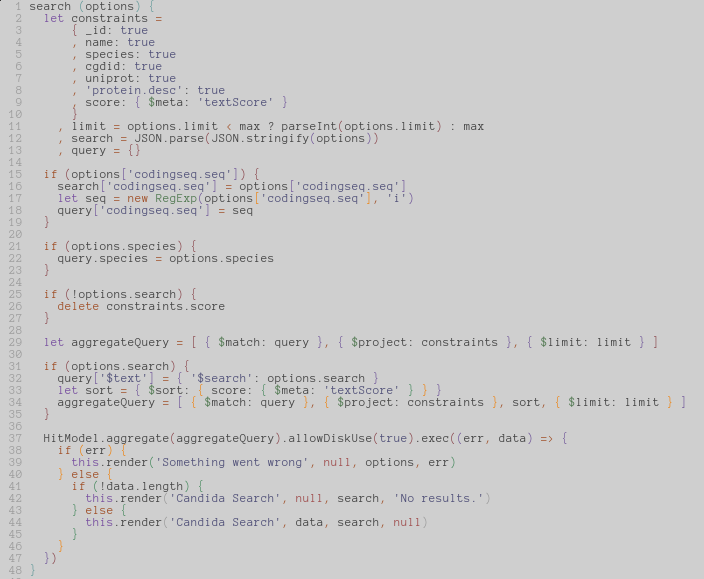
\includegraphics[scale=0.60]{code3}
\caption{Function responsible for creating the aggregate search query. \label{overflow}}
\end{center}
\end{figure}

This fixed the sorting bug, and ensures that all of the correct results for a query are returned, while still maintaining a high level of performance. 

\section{Testing}
Initially it was planned to develop this application in a test driven manner, as it can help to produce high quality code with fewer defects that code produced in a traditional style.\cite{tdd} It also ensures that tests for the project do in fact get written, which often isn't the case when they are written after functionality has been achieved. 

The difficulty with this approach was that when developing prototypes, rapid development is key, as it allows for many different solutions to be tested quickly. If a strict TDD pattern was followed during this phase the prototyping would have been drastically slowed as the amount of development work would have doubled, due to the need to write robust unit tests prior to making the functionality. Unfortunately this wasn't a worthy endeavour as time was limited and developing tests for prototype code that may never end up in the final codebase was not going to be feasible.

Another difficulty in testing this project was that the majority of the projects logic is in the seed script that imports the data into the database. Testing this would be difficult because the only way of really checking the validity of what it was producing was to look at what was in the database and to see if that made sense in a biological context. 

Unfortunately it would be beyond the scope of this project to test the biological accuracy of the data that was imported. However I was able to manually verify that the data was correct at several stages, by aligning sequences from this project against other genomic databases such as the Candida Genome Database\cite{cgd} and the Yeast Genome\cite{sgd} project. 

\subsection{Automated Testing}
For the area's of logic that were testable, a TDD design was followed, mainly for the selection of the coding sequence in the contig, as this was the only real area of logic in the project that had it's own custom algorithm to be tested. In addition to this the test suite that was being used for the project also checked the project for code formatting issues with the ESLint\cite{eslint} tool. This will cause the tests to fail if potentially dangerous assertions are made in the code. For example if an equal to value (==) operator was used instead of an equal to value and type (===) operator it will throw an error highlighting the issue to the developer. 

\subsubsection{Unit Tests}
Where possible, test driven development was used to produce unit tests, these were mainly written for the logic that detects the coding sequence inside the contig. This is a crucial algorithm as the sites functionality depends on this data being accurate, so it was important that the algorithm be thoroughly tested. To do this several mock database records were created that had all the different possibilities that a gene could be found in, a normal hit, a reverse compliment hit, a missing hit and a hit that was split above and below the contig. 

Tests were then written to compare the result of the finding function against the correct values stored in the mock data. The function was then able to be developed ensuring that the data it was returning was correct. 

\subsection{User Interface Testing}
The user interface hasn't had automated tests written for it unfortunately, as there was only one HTML page and only two sets of data that were being returned it didn't feel particularly necessary to write tests to check that the data was coming through correctly. 

That being said the UI has been manually tested on Chrome, Firefox and Internet Explorer to check for any functional issues. None were found, however it was noted that in Internet Explorer and Firefox there was some font rendering issues, but this isn't a concern as it doesn't impact the functionality of the site. I will be recommending that the site is used on Chrome though, as that it was it was developed on, so is the most thoroughly tested, with no apparent styling issues. 

Once the site was at a stage where it could be demonstrated, the UI was shown to the researchers and they were asked to provide any feedback that might make the site easier to use for them. This feedback was mainly focussed on producing a splash page that would act as the home page for external users who were not familiar with the project, data or system. They requested that the University logo be included on the page as well as some text, which has yet to be provided.

\subsection{Stress Testing}
As this site is hosting commercially sensitive data, it won't be publicly accessible, this means that only the researchers who are working on this data will be accessing it. Because of this there isn't a need to perform any stress testing on the service, as the stack is more than capable of handling \textless 10 users at a time, and isn't vulnerable to public attacks. To help combat any potential risks of stress on the system a Varnish\cite{varnish} cache will be placed in front of the service to cache common requests, thus reducing the load on the server. 

\subsection{Integration Testing}
As discussed in the build process section (2.3), continuous integration services were used throughout this project, meaning that every time a new build was pushed to Github, it had to pass tests on the CI server before being deployed to the staging server on Heroku. This has ensured that any modifications to the code base won't break the core functionality of the staging build. 

\subsection{User Testing}
Once the site had been developed to a stage where the users can get a real sense of how it is looking and how it will function, they were invited to suggest changes that need to be made, in line with the agile practices that this project has been developed with. 

User testing was invaluable as the researchers were able to spot mistakes in the biological data that had previously gone unnoticed. An instance of this is when they noted that one of the UniProt IDs was linking to a gene found in the flu virus, something that shouldn't be present at all in the yeast genome. After investigating, it was found that some of the UniProt IDs had been truncated which caused this anomaly. Writing tests for these kinds of checks would have been nigh on impossible, thankfully user testing was able to pick up these kinds of issues. 
